% REVISÃO DE LITERATURA--------------------------------------------------------

\chapter{REFERENCIAL TEÓRICO}
\label{chap:fundamentacaoTeorica}

O sistema que se pretende desenvolver é fundamentalmente colaborativo, \citeonline{Alcantara2016} , tratando de colaboração entre empresas diz que elas trabalham em conjunto para obter um resultado melhor do que o que seria possível trabalhando separadamente. Esta é também a proposta do projeto, pois as universidades não necessitariam de fazer as traduções, apenas validar as que tenham sido realizadas e os alunos teriam uma fonte confiável de consulta, pois, não estariam se submetendo apenas à tradução de seus pares, mas, a uma tradução com qualidade comprovada por uma instituição de ensino reconhecida.

“A colaboração ocorre quando entidades concordam na determinação de objetivos definidos e usam seus recursos (informações, pessoas, tecnologias) para criar sinergias e alcançar vantagem competitiva a longo prazo” \cite{Alcantara2016}

\citeonline{Greef2014} ressaltam que o trabalho colaborativo não apresenta uma hierarquia, as partes assumem responsabilidade sobre as atividades a serem realizadas e confiam umas nas outras na condução das ações.

Embora a confiança seja uma característica marcante de um processo colaborativo, ela é delicada, \citeonline{Greef2014} apontam fenômenos que levam a perdas de motivação e de coordenação em projetos colaborativos:

\begin{itemize}
	\item \textbf{Social loafing}: Quando o indivíduo não se empenha tanto trabalhando em grupo como quando trabalha só
	\item \textbf{Free-riding}: Quando o indivíduo não contribui, mas, se beneficia do projeto 
	\item \textbf{Sucker-effect}: Quando um indivíduo que contribui nota a existência de free-riding, por parte dos outros componentes do grupo de trabalho
	\item \textbf{Efeito Ringelman}: É definido como inatividade social, pode ser entendido como o resultado dos três fenômenos acima, indica uma tendência à redução de produtividade de pessoas quando trabalham em conjunto e que esta tendência aumenta proporcionalmente ao tamanho do grupo de trabalho
\end{itemize}

Deixar evidente o nível de colaboração de cada membro, quantitativa e qualitativamente, usando um padrão justo para avaliação da contribuição de cada participante é um modo de reduzir o social loafing, de acordo com \citeonline{Greef2014}. Nota-se também que esta atitude pode ter efeito positivo sobre o Free-riding e consequentemente sobre o Free-riding e Efeito Ringelman, possibilitando uma maior produtividade dos envolvidos no projeto.

\citeonline{Greef2014} apresentam uma série de dificuldades que podem ser enfrentadas no desenvolvimento de um projeto colaborativo, considerando estas dificuldades, a realização desta pesquisa se mostrou evidentemente necessária antes da criação de uma estrutura complexa que dependerá completamente do sucesso do colaborativismo entre alunos e instituições de ensino.

Em seu trabalho \citeonline{Greef2014} tratam da produção colaborativa de textos em uma ferramenta \textit{wiki} e adotam um princípio que é representado pelo quadro na figura abaixo:

\begin{figure}[!htb]
	\centering
	\caption{Princípio cooperativo de Grice}
	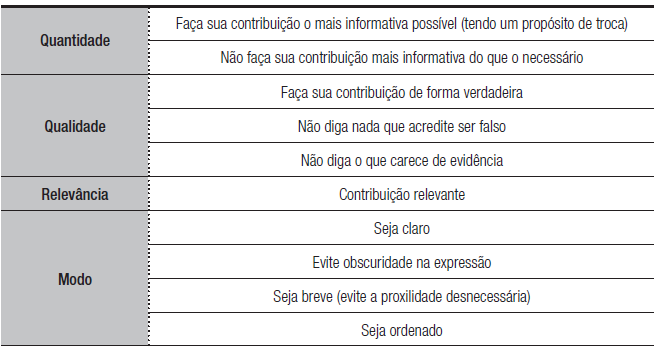
\includegraphics[width=1.0\textwidth]{./dados/figuras/distribuicao-grice}
	\fonte{\citeonline{Greef2014}}
	\label{fig:quadro-grice}
\end{figure}

A divisão no quadro é muito adequada para um contexto como o da construção de texto de forma colaborativa onde há a possibilidade de comentários de diversas pessoas, o que é um pouco diferente da proposta do projeto de traduções, porém, também e aplicável levando em conta que o responsável pela tradução deve seguir este mesmo princípio para produzir um texto que seja uma tradução adequada, mas, que também seja claro e de fácil entendimento, e o responsável pela validação das traduções também deve se limitar a garantir estas características, sem se envolver em “rodeios” que não contribuam para a democratização do conhecimento contido no documento traduzido.

\citeonline{Greef2014} ainda chamam a atenção para o risco de que de forma não intencional, as atitudes de algum participante do processo possa produzir problemas em relação aos outros. Um exemplo poderia ser a não aprovação de uma tradução ou uma crítica a algum problema encontrado em uma tradução já realizada.

O resultado desta pesquisa pode promover um incentivo à comunidade acadêmica para se envolver na redução da barreira linguística e facilitar o acesso a informação.

